\documentclass[man, 10pt]{apa7}
\usepackage[spanish]{babel}
\usepackage{graphfig}
\usepackage{minted} % para código
\usepackage[utf8]{inputenc}
\usepackage{csquotes}
\usepackage{float}
\usepackage{placeins}
\usepackage{capt-of}


\usepackage[style=apa, backend=biber, sortcites=true, doi=true, isbn=false, url=true]{biblatex}
\addbibresource{bibliografia.bib}
\setcounter{secnumdepth}{3}

% título
\title{\scshape {Software como Servicio para la automatización de mensajería y optimización de la comunicación institucional mediante agentes de autorespuesta}}
\shorttitle{}
\author{Marthel Pedro Pozo Solíz \\ Melissa Shanner Nuñez Ardaya}
\date{\today}

\begin{document}
\hypersetup{pageanchor=false}
\begin{titlepage}
	\centering
    \begin{minipage}[c]{0.10\textwidth}
        \centering
        
\includegraphics[width=0.80\textwidth]{./img/logo.png}
    \end{minipage}
    \hfill
    \begin{minipage}[c]{0.70\textwidth}
        \centering
        {\scshape\large Universidad Autonoma Gabriel Rene Moreno \par}
        {\scshape\Large Facultad de Integral del Chaco\par}
        {\scshape\large Ingenieria Informatica - Ingenieria en Sistemas\par}
    \end{minipage}
    \hfill
    \begin{minipage}[c]{0.10\textwidth}
        \centering
        
\includegraphics[width=0.80\textwidth]{./img/logo2.png}
    \end{minipage}\par
    \vspace{3cm}
    {\LARGE\textbf{
    Propuesta para la Implementacion de un Servicio para la Automatización de Mensajería y Optimización de la Comunicación Institucional}\par}
    \vspace{1cm}

	Materia: {\Large \itshape \textbf{Preparacion y Evaluacion de Proyecto     ECO449} \par}
	Docente: {\Large \textbf{Msc. Lic. Ofman Blanco Pacheco}\par}
	\vspace{1cm}
	Estudiantes: \\ 
	{\Large \textbf{Nuñez Ardaya Melissa Shanner - 222106301} \par}
	{\Large \textbf{Plata Segovia Cristian - 220121583} \par}
	{\Large \textbf{Pozo Solíz Marthel Pedro - 222106867} \par}
    \vfill

    \vspace{1cm}
	Gestion 1-2026\par
    Camiri, \today
\end{titlepage}


\tableofcontents
\listoffigures
\listoftables
\newpage
\pagenumbering{arabic}
\setcounter{page}{1}
\hypersetup{pageanchor=true}

% \input{./secciones/00_resumen.tex}%
\section{Perfil}
\subsection{Introducción}

En la actualidad, el uso de tecnologías digitales se ha convertido en un elemento fundamental para el desarrollo y crecimiento de los negocios. La transformación digital ha permitido que empresas y emprendimientos adopten nuevas herramientas que facilitan la comunicación con los clientes, optimizan los procesos de atención y mejoran la eficiencia en la gestión de la información. En este contexto, las aplicaciones de mensajería instantánea como WhatsApp y Telegram se han consolidado como uno de los principales canales de interacción entre empresas y usuarios, debido a su facilidad de uso, accesibilidad y amplia presencia en la vida cotidiana de las personas.

Sin embargo, muchos negocios aún gestionan la atención a sus clientes de forma manual, lo que puede generar retrasos en las respuestas, saturación de mensajes y dificultades para brindar información oportuna. Esta situación se vuelve más evidente cuando el volumen de consultas aumenta, provocando una disminución en la calidad del servicio y, en algunos casos, la pérdida de posibles clientes.

Ante esta problemática, el desarrollo de sistemas automatizados basados en bots conversacionales representa una alternativa eficiente para mejorar la atención digital. Estas herramientas permiten automatizar respuestas frecuentes, brindar información inmediata y mantener una comunicación constante con los usuarios, reduciendo la carga operativa y optimizando el tiempo de respuesta.

El presente proyecto propone el desarrollo un bot automatizado integrado a las plataformas de WhatsApp y Telegram, diseñado para responder consultas de manera inmediata y facilitar la interacción entre los negocios y sus clientes. El sistema permitirá gestionar mensajes automáticos, proporcionar información relevante y apoyar en la atención digital, contribuyendo a mejorar la experiencia del usuario y la eficiencia en la comunicación empresarial.
\subsection{Planteamiento del Problema}

Las organizaciones que atienden consultas por canales de mensajería, como universidades, empresas, tiendas, centros de servicios y entidades públicas, enfrentan dificultades recurrentes en su comunicación institucional digital con estudiantes, clientes, ciudadanos o beneficiarios.

En este entorno, estas instituciones y negocios reciben un alto volumen de consultas repetitivas sobre horarios, requisitos, estados de trámite, precios, disponibilidad, costos, fechas clave y soporte operativo. La gestión manual de estas interacciones suele generar demoras en la respuesta, saturación del personal, inconsistencias en la información y baja trazabilidad del historial conversacional.

El problema se intensifica cuando existen múltiples canales no integrados, porque se duplican esfuerzos y se dificulta mantener criterios unificados de atención. Además, la falta de automatización limita la capacidad de ofrecer respuestas oportunas fuera del horario laboral, afectando la experiencia del usuario y la percepción de calidad del servicio.

En consecuencia, el problema central consiste en la ausencia de una solución \textit{Software como Servicio (SaaS)} que centralice conversaciones, automatice respuestas frecuentes y optimice los flujos de comunicación con control, escalabilidad y consistencia informativa.
\subsubsection{Formulación del Problema}
¿Cómo mejorar la atención y gestión de consultas de los usuarios mediante la implementación de un sistema automatizado de respuestas integrado en plataformas de mensajería como WhatsApp y Telegram?
%\input{secciones/99-antecedentes.tex}
\subsection{Justificación}
El crecimiento del uso de plataformas de mensajería instantánea ha transformado la forma en que las organizaciones interactúan con sus usuarios. Actualmente, canales como WhatsApp y Telegram se han convertido en medios de comunicación fundamentales para la atención al cliente, soporte técnico y gestión de consultas informativas. Sin embargo, muchas instituciones y negocios continúan gestionando estas interacciones de manera manual, lo que provoca retrasos en la respuesta, sobrecarga del personal y dificultades para mantener la consistencia en la información proporcionada.

En este contexto, el desarrollo de una plataforma basada en Software como Servicio (SaaS) que permita automatizar la atención mediante flujos de respuesta representa una solución tecnológica viable. Este tipo de sistemas permite responder de forma inmediata a preguntas frecuentes, reducir la carga operativa del personal y mejorar la disponibilidad del servicio, incluso fuera del horario laboral.

La integración de múltiples canales de mensajería dentro de una misma plataforma facilita la centralización de conversaciones, el seguimiento de consultas y la gestión eficiente de la información. En términos de adopción de mercado, WhatsApp mantiene una posición dominante a nivel global, con aproximadamente 3.000 millones de usuarios activos mensuales en octubre de 2025 \parencite{statista_messaging_2025}. Asimismo, Statista reporta 1,53 mil millones de usuarios que interactúan vía WhatsApp Business en 2023 y un ARPU aproximado de 0,25 dólares estadounidenses para ese mismo periodo \parencite{statista_whatsapp_business_2023}. Por su parte, Telegram alcanza aproximadamente 1.000 millones de usuarios activos y se posiciona como la tercera plataforma de mensajería más utilizada.

De acuerdo con LiveConnect, en su estudio sobre adopción de WhatsApp e Instagram en pymes de Latinoamérica \parencite{liveconnect_adopcion_2025}, a nivel mundial se reportan 200 millones de pymes que utilizan WhatsApp Business. Además, con base en un estudio de BCG y Meta en países en vías de desarrollo, se señala que el 75\% de las empresas utiliza WhatsApp durante todo el ciclo de vida del cliente, con liderazgo de mercados como México y Brasil. En Argentina, un estudio de 2023 encontró que el 73\% de emprendedores y pymes eran usuarios de WhatsApp, mientras que en Colombia la adopción alcanzó el 92,2\%.

\subsubsection{Justificación Económica}
La transformación digital constituye un pilar fundamental para el desarrollo económico de los países en la actualidad. En este contexto, el desarrollo de herramientas tecnológicas que faciliten la automatización de procesos de atención representa una contribución a la productividad y competitividad de la economía nacional.

La adopción de soluciones tecnológicas basadas en plataformas de mensajería automatizadas permite a las organizaciones aumentar su eficiencia operativa, lo que se traduce en una mejor utilización de los recursos disponibles a nivel nacional. Al reducir los tiempos de espera y optimizar la gestión de consultas, se favorece el incremento de la productividad en diversos sectores económicos que dependen de la atención al cliente.

Asimismo, el fortalecimiento de la infraestructura digital de atención contribuye a la inclusión tecnológica de pequeñas y medianas empresas, permitiendo que negocios de menor escala puedan acceder a herramientas de automatización que anteriormente estaban disponibles solo para grandes corporaciones. Esta democratización del acceso tecnológico favorece la equidad en el ecosistema empresarial nacional y promueve una distribución más equilibrada de los beneficios de la transformación digital.

De igual manera, la implementación de sistemas automatizados de atención mediante plataformas de mensajería contribuye a reducir la brecha digital entre los diferentes sectores económicos del país. Al facilitar herramientas accesibles y de bajo costo, se promueve la participación de más actores en la economía digital, lo que fortalece el tejido productivo nacional y contribuye al desarrollo económico inclusivo.
\subsubsection{Justificación Social }
El acceso rápido a la información y la atención oportuna se han convertido en aspectos importantes dentro de la comunicación digital actual. Muchas personas utilizan aplicaciones de mensajería instantánea como WhatsApp y Telegram para realizar consultas, solicitar servicios o comunicarse con diferentes organizaciones y negocios.

En este contexto, la implementación de herramientas tecnológicas que permitan mejorar la atención al usuario contribuye a facilitar la comunicación y el acceso a la información. El uso de sistemas automatizados de respuesta permite brindar atención inmediata a las consultas más frecuentes, mejorando la experiencia de los usuarios y reduciendo los tiempos de espera.

De esta manera, el desarrollo de la plataforma propuesta aporta una solución que favorece tanto a los usuarios como a los negocios o instituciones que ofrecen servicios, permitiendo una interacción más rápida, organizada y accesible mediante plataformas de mensajería ampliamente utilizadas.
\subsubsection{Justificación Técnica }

La implementación del sistema propuesto es técnicamente viable debido a la disponibilidad de herramientas de desarrollo, bibliotecas de programación y servicios de integración que permiten conectar aplicaciones con plataformas de mensajería como WhatsApp y Telegram. Estas tecnologías permiten diseñar sistemas capaces de procesar mensajes, generar respuestas automáticas y gestionar múltiples consultas de manera simultánea.

Asimismo, el desarrollo de este tipo de soluciones puede realizarse mediante el uso de arquitecturas de software modernas que facilitan la escalabilidad, el mantenimiento y la integración con otros sistemas digitales. Por lo tanto, el proyecto propuesto se fundamenta en el uso de tecnologías accesibles y ampliamente utilizadas en el ámbito del desarrollo de software, lo que garantiza su factibilidad técnica y su correcta implementación.

\subsection{Objetivo general}
Proponer la implementación de un servicio para la automatización de la mensajería que optimizará la comunicación institucional en canales de mensajería instantánea. Propuesta que se desarrollará entre las fechas 23 de febrero y 11 de julio de 2026.

\subsubsection{Objetivos específicos}
\begin{itemize}
    \item Analizar las necesidades de comunicación digital de organizaciones y negocios que utilizan plataformas de mensajería instantánea para la atención a usuarios.

    \item Definir la localización del proyecto considerando el entorno geográfico, institucional y tecnológico en el que se implementará la plataforma.

    \item Determinar el tamaño del proyecto en función de su alcance operativo, volumen estimado de usuarios y capacidad requerida de procesamiento de mensajes.

    \item Diseñar las partes funcionales del proyecto, definiendo los módulos principales de integración, arquitectura de la plataforma, gestión de conversaciones, automatización de respuestas y administración del sistema.

    \item Analizar la inversión requerida para el proyecto, considerando costos de desarrollo, infraestructura, implementación y operación inicial.

    \item Estimar los ingresos proyectados y los costos operativos del servicio para evaluar su sostenibilidad financiera.

    \item Realizar la evaluación económica, financiera y técnica del proyecto.
\end{itemize}

%\section{Alcance}
El presente proyecto contempla el diseño y desarrollo de una plataforma de mensajería automatizada basada en el modelo Software como Servicio (SaaS), orientada a mejorar la atención digital de organizaciones, negocios y centros de servicio mediante la integración de bots conversacionales en canales de mensajería.

La solución permitirá centralizar la comunicación proveniente de plataformas como WhatsApp y Telegram, automatizar respuestas a consultas frecuentes y ofrecer herramientas de gestión para administrar conversaciones desde una interfaz web.

El sistema incluirá funcionalidades como la configuración de respuestas automáticas, registro del historial de mensajes, administración de usuarios y monitoreo básico de interacciones. Asimismo, se contempla la implementación de tecnologías web modernas para garantizar escalabilidad, seguridad y facilidad de mantenimiento.
\subsection{Localización }
El proyecto se desarrolla en la ciudad de Camiri, departamento de Santa Cruz, Bolivia. Al tratarse de una plataforma digital, su aplicación puede extenderse a diferentes organizaciones o negocios que utilicen servicios de mensajería para la atención a usuarios.
\subsection{Marco teórico}

\subsubsection{Antecedentes de la investigación }

\cite{linocruz2023}, \textit{Implementación de una plataforma de chatbot gestionado por WhatsApp y Telegram para su comercialización en la empresa Innovus Software}, desarrollada en la Universidad Estatal del Sur de Manabí (UNESUM), en Jipijapa.

Este trabajo se centra en la mejora de la atención al cliente mediante un servicio de mensajería automática, orientado a responder consultas frecuentes de forma inmediata y precisa. A nivel metodológico, el estudio emplea revisión bibliográfica, análisis documental, enfoque histórico-lógico y observación del comportamiento de las consultas realizadas por los clientes.

Entre sus principales hallazgos, se reporta que una parte importante de las preguntas recibidas por la empresa son repetitivas y objetivas, lo que justifica la automatización del proceso de respuesta. La propuesta técnica se apoya en librerías (WhatsApp Cloud API) para la escucha de eventos de mensajería y en un algoritmo de secuencias programadas para identificar mensajes y generar respuestas automáticas.

Como resultado, la investigación concluye que la implementación de una plataforma de chatbot en canales como WhatsApp y Telegram contribuye a reducir costos operativos, incrementar la productividad y habilitar un servicio tecnológicamente viable para su comercialización a terceros. Este antecedente respalda la pertinencia del presente proyecto, especialmente en su enfoque de automatización de la comunicación para organizaciones, tiendas y negocios con alta demanda de atención digital.

\cite{vargasbraga_ifc}, en su trabajo \textit{Implementa{\c{c}}{\~a}o de assistente virtual via WhatsApp para aprimorar a comunica{\c{c}}{\~a}o no IFC -- Campus Sombrio}, presentan el desarrollo de un asistente virtual orientado a fortalecer la comunicaci{\'o}n institucional y la difusi{\'o}n de informaci{\'o}n oficial del campus. La propuesta se enfoca en responder dudas generales de los usuarios (por ejemplo, cursos, docentes y ubicaci{\'o}n), y se enmarca como una investigaci{\'o}n tecnol{\'o}gica basada en la construcci{\'o}n de un artefacto funcional. T{\'e}cnicamente, el sistema fue implementado con JavaScript/TypeScript e integrado con la API Baileys para la conexi{\'o}n con WhatsApp. Como resultado, reportan un asistente capaz de entregar respuestas simples de forma m{\'a}s r{\'a}pida que la b{\'u}squeda tradicional en redes sociales o en la web, destacando adem{\'a}s su potencial de ampliaci{\'o}n con nuevas funcionalidades.


\cite{zarabanda2024desarrollo} plantea el desarrollo de un chatbot interactivo para el proyecto curricular de Ingenier{\'i}a Telem{\'a}tica y Sistematizaci{\'o}n de Datos de la Universidad Distrital Francisco Jos{\'e} de Caldas, con el prop{\'o}sito de mejorar la comunicaci{\'o}n entre estudiantes y personal administrativo por medio de WhatsApp. La propuesta contempla funcionalidades orientadas a la gesti{\'o}n de tr{\'a}mites de radicaci{\'o}n de anteproyectos, notificaci{\'o}n de fechas clave, actualizaci{\'o}n de enlaces para documentaci{\'o}n requerida y atenci{\'o}n de preguntas frecuentes. A nivel arquitect{\'o}nico, el dise{\~n}o prioriza modularidad y escalabilidad: los mensajes son gestionados con Baileys y procesados en un servidor Node.js, que a su vez puede consultar MariaDB y APIs externas para construir respuestas adecuadas. Adem{\'a}s, el proyecto adopta metodolog{\'i}a SCRUM, con roles definidos (Product Owner, Scrum M{\'a}ster y equipo de desarrollo) y trabajo organizado en sprints con entregables progresivos desde la configuraci{\'o}n inicial hasta el despliegue y mantenimiento.

\cite{elsen2025hijab} desarrollan una aplicaci{\'o}n web de cat{\'a}logo electr{\'o}nico de productos hiyab integrada con un chatbot de WhatsApp para fortalecer la atenci{\'o}n al cliente en una MIPYME del sector moda musulmana en Indonesia. El estudio atiende problemas de gesti{\'o}n manual de inventario y baja capacidad de respuesta administrativa, proponiendo un sistema que permite consultar detalles de productos, precios, stock en tiempo real y promociones, adem{\'a}s de gestionar pedidos. El chatbot, implementado con la API Baileys, responde consultas frecuentes como ubicaci{\'o}n de tienda y valoraciones de productos, reduciendo carga operativa. La validaci{\'o}n reporta resultados satisfactorios de usabilidad (SUS 71.3 para no clientes y 73.5 para clientes), lo que respalda la pertinencia de integrar cat{\'a}logos web y agentes conversacionales para mejorar eficiencia operativa y experiencia de usuario.


\cite{vega2023nlp}, en su tesis de grado de la Universidad Mayor de San Andr{\'e}s, analiza el uso de procesamiento de lenguaje natural con modelos inteligentes para la atenci{\'o}n de consultas mediante redes sociales. El estudio describe la aplicaci{\'o}n de redes neuronales artificiales y arquitecturas Transformer para mejorar la comprensi{\'o}n del lenguaje en chatbots, con el objetivo de ofrecer interacciones m{\'a}s naturales y efectivas con los usuarios. Como caso aplicado, propone un chatbot para el gimnasio CrossFit capaz de informar sobre horarios, precios, actividades y recomendaciones de entrenamiento y nutrici{\'o}n. Entre los resultados comparativos, reporta mejor desempe{\~n}o del modelo de red neuronal artificial frente a GPT-2 y GPT-3 dentro de la metodolog{\'i}a empleada. Este antecedente aporta evidencia sobre la pertinencia de combinar t{\'e}cnicas de IA y PLN para fortalecer canales de atenci{\'o}n digital.

\subsubsection{Bases Teóricas}

\paragraph{1. Transformación Digital y Comunicación Institucional}
La transformación digital rediseña procesos, canales y decisiones institucionales, habilitando comunicación continua, ágil y centrada en usuarios con expectativas crecientes de inmediatez.

\paragraph{2. Software como Servicio (SaaS)}
Sofware en la nube accedido por suscripción, con escalabilidad, actualizaciones centralizadas y menor inversión inicial para organizaciones sin infraestructura propia.

\paragraph{3. Sistemas Conversacionales y Agentes de Autorespuesta}
Los agentes conversacionales automatizan consultas frecuentes, clasifican intenciones y responden consistentemente, reduciendo carga operativa y derivando casos complejos a atención humana.

\paragraph{4. Integración Multicanal: WhatsApp y Telegram}
La integración multicanal unifica interacciones de WhatsApp y Telegram, mejora trazabilidad, evita fragmentación informativa y sostiene experiencias coherentes en distintos puntos de contacto.

\paragraph{5. Arquitectura Orientada a Servicios y APIs}
Una arquitectura orientada a servicios desacopla módulos mediante APIs, favorece interoperabilidad, escalabilidad y mantenimiento evolutivo, incorporando funciones sin rediseñar todo el sistema.

\paragraph{6. Calidad de Servicio en la Atención Digital}
La calidad digital se mide con tiempos de respuesta, consistencia, disponibilidad y satisfacción; su optimización fortalece confianza institucional y eficiencia operativa sostenida.

\paragraph{7. Experiencia de Usuario (UX) en Canales Conversacionales}
La UX conversacional exige mensajes claros, pertinentes y breves, minimizando fricción comunicacional y facilitando transiciones fluidas hacia atención humana cuando corresponda.

\paragraph{8. Seguridad, Privacidad y Protección de Datos}
La plataforma debe garantizar confidencialidad, integridad y disponibilidad, aplicando controles de acceso, cifrado, trazabilidad y cumplimiento normativo sobre datos sensibles conversacionales.

\paragraph{9. Procesamiento de Lenguaje Natural (PLN) en Chatbots}
El PLN permite reconocer intenciones y entidades en mensajes, mejorando precisión de respuestas y habilitando automatización contextual en dominios institucionales específicos.

\paragraph{10. Evaluación del Rendimiento del Sistema}
El rendimiento se evalúa con KPIs como tiempo de respuesta, resolución automática, abandono, satisfacción y disponibilidad, orientando decisiones de mejora continua.

En síntesis, estas bases teóricas articulan tecnología, gestión y servicio para sustentar una plataforma SaaS de mensajería institucional eficiente, segura y escalable.

\subsubsection{Marco Conceptual}

\begin{itemize}
    \item \textbf{SaaS (Software as a Service).} Modelo de distribución de software en el que las aplicaciones se alojan en servidores de nube y se ofrecen a través de internet bajo suscripción, sin instalación local (\cite{mellgrance2011}).

    \item \textbf{Bot conversacional / Chatbot.} Programa informático diseñado para simular conversaciones con personas mediante lenguaje natural o flujos de diálogo estructurados, procesando mensajes y generando respuestas automáticas (\cite{adamopoulou2020}).

    \item \textbf{Agente de autorespuesta.} Tipo de chatbot orientado a atención institucional o comercial, que responde consultas frecuentes de forma autónoma y escala a operador humano cuando es necesario.

    \item \textbf{API (Application Programming Interface).} Conjunto de definiciones y protocolos que habilita la comunicación e integración entre sistemas de software para intercambiar datos y funcionalidades (\cite{fielding2000}).

    \item \textbf{Baileys (WhatsApp Web API).} Biblioteca de JavaScript/TypeScript que permite integrar WhatsApp Web de forma programática para enviar, recibir y gestionar mensajes automatizados.

    \item \textbf{Telegram Bot API.} API pública y gratuita de Telegram para crear bots que interactúan con usuarios, procesan mensajes, envían multimedia y ejecutan comandos en la plataforma (\cite{telegram2024}).

    \item \textbf{PLN (Procesamiento de Lenguaje Natural).} Rama de la inteligencia artificial que estudia la interacción entre computadoras y lenguaje humano para comprender, interpretar y generar texto significativo (\cite{manningschutze1999}).

    \item \textbf{Omnicanalidad.} Estrategia que garantiza una experiencia de usuario coherente y continua, independientemente del canal utilizado, unificando historiales y criterios de atención (\cite{rigby2011}).

    \item \textbf{Multitenencia (Multitenancy).} Arquitectura donde una misma instancia de aplicación atiende múltiples clientes de forma aislada y segura, compartiendo eficientemente recursos de infraestructura (\cite{armbrust2010}).

    \item \textbf{Trazabilidad conversacional.} Capacidad del sistema para registrar y recuperar el historial completo de interacciones, facilitando auditorías, análisis de comportamiento y continuidad de atención.

    \item \textbf{Escalabilidad.} Propiedad del sistema para incrementar capacidad de procesamiento o usuarios atendidos conforme aumenta la carga, sin degradar rendimiento ni rediseñar la arquitectura.

    \item \textbf{Handoff (Transferencia de canal).} Proceso mediante el cual una conversación automatizada se transfiere a un operador humano, preservando contexto e historial para asegurar continuidad (\cite{folstadskjuve2019}).

    \item \textbf{CSAT (Customer Satisfaction Score).} Indicador de satisfacción obtenido mediante encuestas breves posteriores a la interacción, que mide valoración del usuario en escala numérica definida.

    \item \textbf{Tríada CIA (Confidencialidad, Integridad, Disponibilidad).} Marco de seguridad de la información que establece acceso autorizado, exactitud de datos y disponibilidad oportuna de la información (\cite{iso27001_2022}).
\end{itemize}
\subsection{Metodología de la Investigación}



\subsubsection{Marco legal del proyecto}
El proyecto se enmarca en normativa técnica y jurídica aplicable al tratamiento de información, prestación de servicios digitales y seguridad de la información.

\paragraph{Normativa internacional}
\begin{itemize}
    \item \textbf{ISO/IEC 27001}: Sistema de gestión de seguridad de la información (SGSI), aplicable para definir políticas, controles y gestión de riesgos de la plataforma (\cite{iso27001}).
    \item \textbf{ISO/IEC 27017}: Controles de seguridad para servicios en la nube, relevante para la operación del modelo SaaS (\cite{iso27017}).
    \item \textbf{ISO/IEC 27018}: Protección de datos personales en servicios cloud públicos, útil para el tratamiento responsable de datos de usuarios (\cite{iso27018}).
    \item \textbf{ISO/IEC 27701}: Extensión de privacidad sobre ISO/IEC 27001, orientada a la gestión de información personal (PIMS) (\cite{iso27701}).
    \item \textbf{IEEE 29148}: Lineamientos para la ingeniería de requisitos de sistemas y software, aplicable a la definición y trazabilidad de requisitos funcionales y no funcionales (\cite{ieee29148}).
    \item \textbf{IEEE 1012}: Prácticas de verificación y validación de sistemas y software, aplicables a pruebas y control de calidad del proyecto (\cite{ieee1012}).
\end{itemize}

\paragraph{Normativa nacional (Bolivia)}
\begin{itemize}
    \item \textbf{Constitución Política del Estado}: reconoce el derecho a la privacidad, intimidad y protección de datos personales, principios base para la gestión de información de usuarios (\cite{cpe2009}).
    \item \textbf{Ley N\textsuperscript{o} 164 (Ley General de Telecomunicaciones, Tecnologías de Información y Comunicación)}: establece el marco general para servicios TIC y uso de medios electrónicos en el país (\cite{ley164}).
    \item \textbf{Decreto Supremo N\textsuperscript{o} 1793}: reglamenta la Ley N\textsuperscript{o} 164 en aspectos operativos vinculados a telecomunicaciones y TIC (\cite{ds1793}).
    \item \textbf{Ley N\textsuperscript{o} 453 (Ley General de los Derechos de las Usuarias y los Usuarios y de las Consumidoras y los Consumidores)}: aplicable a la calidad de atención, información transparente y mecanismos de reclamo en servicios digitales (\cite{ley453}).
    \item \textbf{Ley N\textsuperscript{o} 1080 (Ciudadanía Digital)}: regula mecanismos de interacción digital con validez en trámites y servicios electrónicos, relevante para autenticación e intercambio digital de información (\cite{ley1080}).
\end{itemize}

Adicionalmente, para la integración con WhatsApp y Telegram, el sistema deberá cumplir los términos de servicio, políticas de plataforma y condiciones de uso de sus APIs oficiales, especialmente en materia de consentimiento, envío de mensajes y tratamiento de datos (\cite{whatsapp_business_terms,telegram_terms}).

\subsection{Cronograma}

El cronograma de actividades se estructura en seis fases principales que abarcan todo el período del 23 de febrero al 11 de julio de 2026. A continuación se describe cada actividad:

\begin{enumerate}
    \item \textbf{Presentación del perfil del proyecto (23 de febrero - 25 de marzo):} Elaboración y presentación del perfil del proyecto, incluyendo la definición del tema, establecimiento de objetivos, análisis de necesidades del mercado, definición de la localización del proyecto y elaboración del anteproyecto para su aprobación.

    \item \textbf{Realización del estudio de mercado (26 de marzo - 29 de abril):} Investigación de campo para recopilar información sobre el mercado objetivo, análisis de la competencia, definición de la demanda potencial y validación de la viabilidad del servicio de mensajería automatizada.

    \item \textbf{Análisis de ingeniería, tamaño, localización y administración (30 de abril - 3 de junio):} Diseño de la arquitectura de la plataforma, definición de módulos del sistema, diseño de agentes de autorrespuesta, definición de la organización del sistema y análisis de tamaño y capacidad del proyecto.

    \item \textbf{Evaluación de inversión, financiamiento, ingresos, costos y evaluación económica (4 de junio - 17 de junio):} Determinación de la inversión requerida, análisis de financiamiento, estimación de ingresos y costos operativos, y evaluación económica mediante indicadores de viabilidad.

    \item \textbf{Preparación de la presentación final (18 de junio - 24 de junio):} Elaboración de la documentación final del proyecto, incluyendo marco teórico, antecedentes, bases metodológicas, resultados y conclusiones.

    \item \textbf{Preparación de defensa final (25 de junio - 6 de julio):} Repaso general del proyecto, preparación de materiales para la defensa y ajustes finales antes de la presentación formal.

    \item \textbf{Entrega del producto (11 de julio):} Presentación y defensa oficial del proyecto final.
\end{enumerate}

\begin{center}
    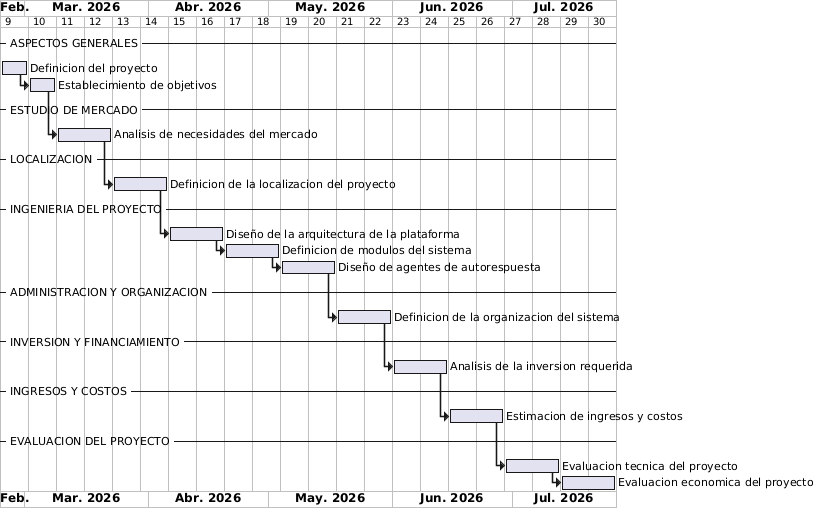
\includegraphics[width=\textwidth]{img/cronograma.png}
    \captionsetup{hypcap=false}
    \captionof{figure}{Cronograma de actividades del proyecto}
    \label{fig:cronograma}
\end{center}
\subsection{Presupuesto}

Estructura referencial del presupuesto para la fase de investigación previa.

\begin{center}
\begin{tabular}{p{0.42\textwidth} c c c }
\hline
\textbf{Concepto} & \textbf{Cantidad} & \textbf{Costo unitario (Bs)} & \textbf{Costo total (Bs)} \\
\hline
Diseño y aplicación de encuestas & -- & -- & -- \\
Entrevistas y levantamiento de información & -- & -- & -- \\
Transporte para trabajo de campo & -- & -- & -- \\
Materiales y suministros (impresiones, papelería) & -- & -- & -- \\
Procesamiento y análisis de datos & -- & -- & -- \\
Comunicación y conectividad (internet/telefonía) & -- & -- & -- \\
Imprevistos (\%) & -- & -- & -- \\
\hline
\multicolumn{3}{|r|}{\textbf{Total general}} & \textbf{--} \\
\hline
\end{tabular}
\captionsetup{hypcap=false}
\captionof{table}{Presupuesto referencial de la investigación previa}
\label{tab:presupuesto-investigacion-previa}
\end{center}

\printbibliography

\end{document}
